\clearpage
%% ============================================================
\section{Pełny loss LeJEPA}
\label{sec:fulloss}
%% ============================================================

\begin{equation}
\boxed{
\mathcal{L}_{\text{LeJEPA}} =
\underbrace{\frac{\lambda}{V} \sum_{v=1}^{V} \mathrm{SIGReg}\!\left(\{\mathbf{z}_{n,v}\}_{n=1}^B\right)}_{\text{regularyzacja: wymuś } \mathcal{N}(\mathbf{0}, \mathbf{I})}
+ \underbrace{\frac{1-\lambda}{B} \sum_{n=1}^{B} \mathcal{L}_{\text{pred}}^{(V_g)}\!\left(\{\mathbf{z}_{n,v}\}_{v=1}^V\right)}_{\text{predykcja: wymuś semantyczną spójność}}
}
\label{eq:lejepa}
\end{equation}

gdzie loss predykcyjny to:
\begin{equation}
\mathcal{L}_{\text{pred}} = \frac{1}{V}\sum_{v'=1}^{V}
\left\|\boldsymbol{\mu}_n - \mathbf{z}_{n,v'}\right\|_2^2,
\quad
\boldsymbol{\mu}_n \triangleq \frac{1}{V_g}\sum_{v=1}^{V_g} \mathbf{z}_{n,v}
\label{eq:pred_loss}
\end{equation}

\begin{keyinsight}[Jeden hiperparametr!]
$\lambda$ kontroluje trade-off między:
\begin{itemize}
  \item $\lambda \to 0$: czysta predykcja (ryzyko kolapsu),
  \item $\lambda \to 1$: czysty SIGReg (brak semantycznej struktury),
  \item $\lambda = 0.05$: \textbf{rekomendowane} — stabilne na wielu datasetach i architekturach.
\end{itemize}
\end{keyinsight}

%% --- Szczegółowe wyjaśnienie wzoru (25) ---
\subsection{Jak czytać wzór (\ref{eq:lejepa}) --- słownik symboli}

Zanim przeczytamy wzór, ustalmy co oznacza \textbf{każdy symbol}:

\begin{center}
\renewcommand{\arraystretch}{1.4}
\begin{tabular}{c p{10cm}}
\toprule
\textbf{Symbol} & \textbf{Znaczenie} \\
\midrule
$\mathcal{L}_{\text{LeJEPA}}$ &
  Pełna \textbf{funkcja straty} (loss) --- jedna liczba, którą sieć minimalizuje
  w~każdym kroku treningu. Im mniejsza, tym lepiej. \\
$\lambda$ &
  \textbf{Hiperparametr balansujący} --- liczba z~przedziału $[0, 1]$
  (typowo $0{.}05$). Kontroluje proporcję:
  ile ``uwagi'' poświęcamy regularyzacji, a~ile predykcji. \\
$V$ &
  \textbf{Liczba wszystkich widoków} (views) jednego obrazu.
  W~LeJEPA: $V = V_g + V_l$, np.\ $V = 2 + 6 = 8$
  (2~globalne + 6~lokalnych). \\
$V_g$ &
  \textbf{Liczba widoków globalnych} (global views) ---
  duże kadrowania ($224 \times 224$) z~jednego obrazu. Typowo $V_g = 2$. \\
$V_l$ &
  \textbf{Liczba widoków lokalnych} (local views) ---
  małe kadrowania ($96 \times 96$). Typowo $V_l = 6$. \\
$B$ &
  \textbf{Rozmiar batcha} --- ile obrazów przetwarzamy na raz
  (np.\ $B = 256$). \\
$n$ &
  \textbf{Indeks obrazu} w~batchu: $n \in \{1, 2, \ldots, B\}$. \\
$v$ &
  \textbf{Indeks widoku}: $v \in \{1, 2, \ldots, V\}$. \\
$\mathbf{z}_{n,v} \in \mathbb{R}^d$ &
  \textbf{Embedding} $n$-tego obrazu z~$v$-tego widoku ---
  wektor $d$-wymiarowy (np.\ $d = 128$) wyprodukowany
  przez sieć (ViT + projektor). \\
$\mathrm{SIGReg}(\cdot)$ &
  Regularyzator z~sekcji~9.5 --- mierzy, jak daleko embeddingi
  są od rozkładu $\mathcal{N}(\mathbf{0}, \mathbf{I})$. \\
$\mathcal{L}_{\text{pred}}$ &
  \textbf{Loss predykcyjny} --- mierzy, jak bardzo embeddingi różnych
  widoków \textit{tego samego} obrazu różnią się od siebie. \\
$\boldsymbol{\mu}_n$ &
  \textbf{Centroid} (średnia) embeddingów widoków globalnych
  $n$-tego obrazu. Punkt odniesienia, do którego
  porównujemy wszystkie widoki. \\
$\|\cdot\|_2^2$ &
  \textbf{Kwadrat normy euklidesowej} --- suma kwadratów
  różnic po współrzędnych: $\|\mathbf{a} - \mathbf{b}\|_2^2 = \sum_i (a_i - b_i)^2$. \\
$\triangleq$ &
  ``\textbf{definiujemy jako}'' --- symbol oznacza, że lewa strona jest
  \textit{nową definicją}, nie wynikiem obliczeń. \\
\bottomrule
\end{tabular}
\end{center}

%% ============================================================
\subsection{Wielowidokowa architektura: globalne i lokalne widoki}
\label{sec:multiview}
%% ============================================================

Zanim przejdziemy do czytania wzoru krok po kroku,
musimy zrozumieć \textbf{kluczowy mechanizm} LeJEPA:
dlaczego sieć nie patrzy na każdy obraz raz, lecz generuje
z~niego wiele \textbf{widoków} (views) --- i~dlaczego dzieli je
na \textbf{globalne} i~\textbf{lokalne}.

%% --- 1. Dlaczego wiele widoków? ---
\subsubsection{Dlaczego wiele widoków? Problem kolapsu i trywialnych rozwiązań}

Wyobraź sobie, że sieć widzi każdy obraz \textbf{dokładnie raz}.
Może wtedy po prostu ``zapamiętać'' każde zdjęcie osobno
--- przypisać mu unikalny wektor --- i~nigdy nie musi uczyć się
\textbf{uogólnionych} cech. To trywialne rozwiązanie nie pomaga
w~żadnym zadaniu downstream (klasyfikacja, detekcja, segmentacja).

\medskip
Wielowidokowość wymusza coś zupełnie innego:

\begin{tcolorbox}[colback=lejepaGreen!8, colframe=lejepaGreen!80, breakable,
  title={\textbf{Wymuszanie inwariantności}}]
Jeśli sieć dostaje \textbf{wiele perspektyw tego samego obiektu}
i~musi produkować dla nich \textbf{bliskie embeddingi},
to \textit{nie może} zapamiętywać pikseli ---
musi wyuczyć się \textbf{abstrakcyjnych cech} (kształt, tekstura, kontekst),
które są \textbf{inwariantne} wobec zmian perspektywy.

\medskip
\textbf{Analogia:} rozpoznajesz kolegę niezależnie od tego,
czy widzisz go z~przodu, z~profilu, z~daleka, czy w~ciemnym pokoju.
Twój mózg wyuczył się \textit{inwariantnej reprezentacji} twarzy
--- i~dokładnie to chcemy osiągnąć dla sieci.
\end{tcolorbox}

Ale jest haczyk --- gdyby sieć mogła produkować \textbf{ten sam wektor}
dla \textit{wszystkich} obrazów (nie tylko widoków tego samego obrazu),
loss predykcyjny byłby zerowy. To \textbf{kolaps} ---
wszystko $\to$ jeden punkt. Dlatego potrzebujemy SIGReg
(sekcja~\ref{sec:sigreg}), który rozpycha embeddingi gaussowsko.

%% --- 2. Globalne vs lokalne — intuicja ---
\subsubsection{Globalne vs lokalne --- intuicja}

Nie wystarczy generować wielu identycznych widoków.
LeJEPA celowo tworzy widoki o~\textbf{różnych skalach}:

\begin{center}
\renewcommand{\arraystretch}{1.3}
\begin{tabular}{lcc}
\toprule
& \textbf{Widoki globalne} & \textbf{Widoki lokalne} \\
\midrule
\textbf{Co widzą?} & cały obiekt / dużą scenę & fragment / detal \\
\textbf{Rozdzielczość} & $224 \times 224$ px & $96 \times 96$ px \\
\textbf{Skala kadrowania} & $0{.}3$--$1{.}0$ obrazu & $0{.}05$--$0{.}3$ obrazu \\
\textbf{Liczba} & $V_g = 2$ & $V_l = 6$ \\
\textbf{Rola w~lossie} & punkt odniesienia (centroid $\boldsymbol{\mu}_n$) & ``uczniowie'' zbliżający się do centroidu \\
\bottomrule
\end{tabular}
\end{center}

\begin{tcolorbox}[colback=blue!4, colframe=blue!60!black, breakable,
  title={\textbf{Dlaczego potrzebujemy obu?}}]
\textbf{Same globalne} --- sieć uczy się kontekstu,
ale nie rozumie lokalnych detali
(np.\ nie rozpozna narzędzia chirurgicznego z~bliska).

\textbf{Same lokalne} --- sieć uczy się detali,
ale traci kontekst
(np.\ nie odróżni fragmentu rogówki od fragmentu tęczówki bez otoczenia).

\textbf{Oba razem} --- sieć musi powiązać ``duży obraz''
z~``małym detalem'' tego samego obiektu.
To wymusza \textbf{hierarchiczne rozumienie} sceny:
od ogółu do szczegółu.
\end{tcolorbox}

Poniższy diagram pokazuje, jak wygląda zestaw widoków
wygenerowanych z~jednego obrazu. Dwa duże niebieskie kadrowania
obejmują znaczną część obrazu (widoki globalne),
a~sześć małych czerwonych kwadratów wycina drobne fragmenty
(widoki lokalne):

\begin{center}
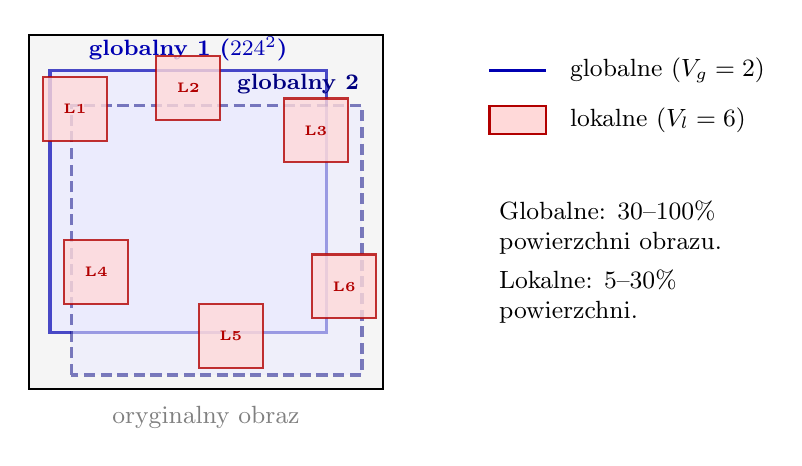
\begin{tikzpicture}[>=stealth, scale=0.9]
  % Oryginalny obraz
  \draw[thick, fill=gray!8] (0,0) rectangle (5,5);
  \node[gray] at (2.5, -0.4) {\small oryginalny obraz};

  % Globalne widoki (duże, niebieskie, przezroczyste)
  \draw[blue!70!black, very thick, fill=blue!8, opacity=0.7]
    (0.3, 0.8) rectangle (4.2, 4.5);
  \node[blue!70!black, font=\footnotesize\bfseries] at (2.25, 4.8)
    {globalny 1 ($224^2$)};

  \draw[blue!50!black, very thick, fill=blue!8, opacity=0.5,
    dash pattern=on 4pt off 2pt]
    (0.6, 0.2) rectangle (4.7, 4.0);
  \node[blue!50!black, font=\footnotesize\bfseries] at (3.8, 4.3)
    {globalny 2};

  % Lokalne widoki (małe, czerwone)
  \foreach \x/\y/\n in {0.2/3.5/1, 1.8/3.8/2, 3.6/3.2/3,
                         0.5/1.2/4, 2.4/0.3/5, 4.0/1.0/6} {
    \draw[red!70!black, thick, fill=red!15, opacity=0.8]
      (\x, \y) rectangle ({\x+0.9}, {\y+0.9});
    \node[red!70!black, font=\tiny\bfseries] at ({\x+0.45}, {\y+0.45})
      {L\n};
  }

  % Legenda
  \draw[blue!70!black, very thick] (6.5, 4.5) -- (7.3, 4.5);
  \node[anchor=west, font=\small] at (7.5, 4.5)
    {globalne ($V_g = 2$)};
  \draw[red!70!black, thick, fill=red!15] (6.5, 3.6) rectangle (7.3, 4.0);
  \node[anchor=west, font=\small] at (7.5, 3.8)
    {lokalne ($V_l = 6$)};

  \node[anchor=north west, align=left, font=\small] at (6.5, 2.8)
    {Globalne: $30$--$100\%$\\powierzchni obrazu.\\[3pt]
     Lokalne: $5$--$30\%$\\powierzchni.};
\end{tikzpicture}
\end{center}

%% --- 3. Jak to działa dla obrazów ---
\subsubsection{Jak to działa dla obrazów (np.\ ImageNet)}
\label{sec:views_images}

Dla pojedynczych zdjęć (nie wideo) \textbf{wszystkie widoki}
powstają z~\textbf{tego samego obrazu} przez pipeline augmentacji:

\begin{center}
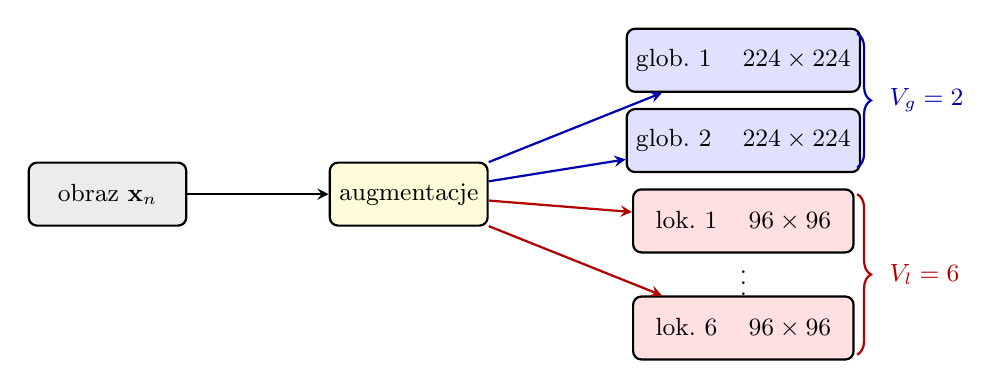
\begin{tikzpicture}[>=stealth, scale=0.85,
  box/.style={draw, thick, rounded corners=3pt, minimum height=0.8cm,
              minimum width=2cm, align=center, font=\small}]

  % Obraz wejściowy
  \node[box, fill=gray!15] (img) at (0, 0) {obraz $\mathbf{x}_n$};

  % Pipeline augmentacji
  \node[box, fill=yellow!15] (aug) at (4.5, 0) {augmentacje};

  % Strzałka
  \draw[->, thick] (img) -- (aug);

  % Widoki globalne
  \node[box, fill=blue!12, minimum width=2.8cm] (g1) at (9.5, 2.0)
    {glob.\ 1 \;\; $224 \times 224$};
  \node[box, fill=blue!12, minimum width=2.8cm] (g2) at (9.5, 0.8)
    {glob.\ 2 \;\; $224 \times 224$};

  % Widoki lokalne
  \node[box, fill=red!12, minimum width=2.8cm] (l1) at (9.5, -0.4)
    {lok.\ 1 \;\; $96 \times 96$};
  \node[font=\small] (dots) at (9.5, -1.2) {$\vdots$};
  \node[box, fill=red!12, minimum width=2.8cm] (l6) at (9.5, -2.0)
    {lok.\ 6 \;\; $96 \times 96$};

  % Strzałki
  \draw[->, thick, blue!70!black] (aug) -- (g1);
  \draw[->, thick, blue!70!black] (aug) -- (g2);
  \draw[->, thick, red!70!black] (aug) -- (l1);
  \draw[->, thick, red!70!black] (aug) -- (l6);

  % Nawiasy
  \draw[decorate, decoration={brace, amplitude=5pt}, blue!70!black, thick]
    (11.2, 2.4) -- (11.2, 0.4) node[midway, right=8pt, blue!70!black,
    font=\small] {$V_g = 2$};
  \draw[decorate, decoration={brace, amplitude=5pt}, red!70!black, thick]
    (11.2, 0.0) -- (11.2, -2.4) node[midway, right=8pt, red!70!black,
    font=\small] {$V_l = 6$};
\end{tikzpicture}
\end{center}

Każdy widok przechodzi \textbf{niezależny} losowy zestaw augmentacji.
Parametry podane poniżej odpowiadają konfiguracji użytej
w~implementacji referencyjnej:

\begin{center}
\renewcommand{\arraystretch}{1.3}
\begin{tabular}{l c c}
\toprule
\textbf{Parametr augmentacji} & \textbf{Globalne} & \textbf{Lokalne} \\
\midrule
Rozdzielczość wyjściowa        & $224 \times 224$ & $96 \times 96$ \\
Skala \texttt{RandomResizedCrop} & $[0{.}3,\; 1{.}0]$ & $[0{.}05,\; 0{.}3]$ \\
Losowy obrót (flip)             & $p = 0{.}5$ & $p = 0{.}5$ \\
Zmiana kolorów (\texttt{ColorJitter}) & jasność, kontrast, nasycenie, barwa & jak globalne \\
\texttt{GaussianBlur}           & $p = 0{.}5$, $\sigma \in [0{.}1,\; 2{.}0]$
                                & $p = 0{.}5$, $\sigma \in [0{.}1,\; 2{.}0]$ \\
Normalizacja                    & \multicolumn{2}{c}{ImageNet: $\mu = (0{.}485,\, 0{.}456,\, 0{.}406)$,
                                  $\sigma = (0{.}229,\, 0{.}224,\, 0{.}225)$} \\
\bottomrule
\end{tabular}
\end{center}

\textbf{Kluczowa różnica} między widokami globalnymi i~lokalnymi
to \textbf{skala kadrowania}: globalne wycinają $30$--$100\%$ obrazu,
lokalne --- zaledwie $5$--$30\%$.
Reszta augmentacji jest taka sama.

%% --- 4. Jak to działa dla wideo ---
\subsubsection{Jak to działa dla wideo (chirurgia katarakty)}
\label{sec:views_video}

Dla danych wideo pipeline jest fundamentalnie inny ---
widoki lokalne powstają z~\textbf{innych klatek} niż widoki globalne.
Wykorzystujemy fakt, że \textbf{czas dostarcza naturalnych transformacji}:

\begin{center}
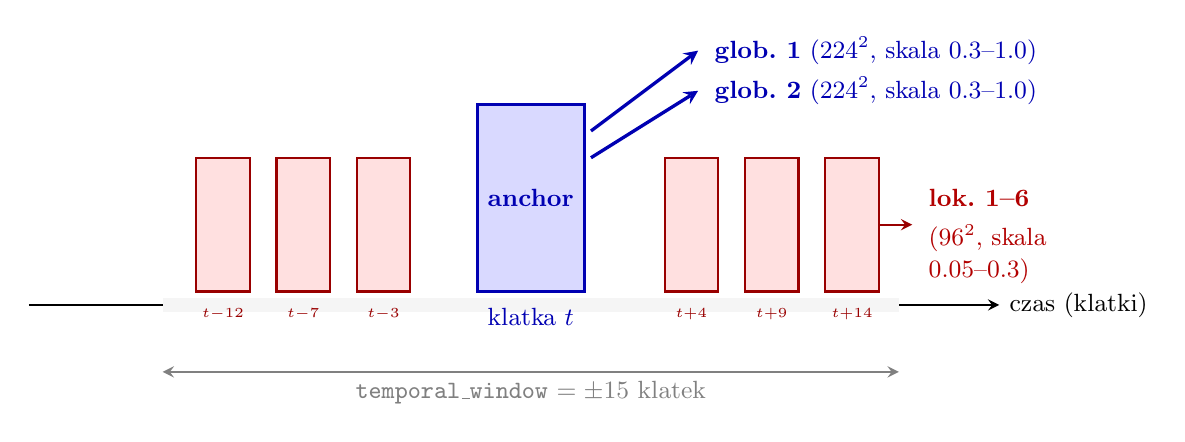
\begin{tikzpicture}[>=stealth, scale=0.85]
  % Oś czasu
  \draw[->, thick] (-0.5, 0) -- (14, 0)
    node[right, font=\small] {czas (klatki)};

  % Okno ±15
  \fill[gray!8] (1.5, -0.1) rectangle (12.5, 0.1);
  \draw[<->, gray, thick] (1.5, -1.0) -- (12.5, -1.0);
  \node[gray, below, font=\small] at (7.0, -1.0)
    {\texttt{temporal\_window} $= \pm 15$ klatek};

  % Klatki sąsiednie (czerwone, źródło widoków lokalnych)
  \foreach \x/\lab in {
    2.0/$t{-}12$, 3.2/$t{-}7$, 4.4/$t{-}3$,
    9.0/$t{+}4$, 10.2/$t{+}9$, 11.4/$t{+}14$} {
    \fill[red!12] (\x, 0.2) rectangle ({\x+0.8}, 2.2);
    \draw[red!60!black, thick] (\x, 0.2) rectangle ({\x+0.8}, 2.2);
    \node[below, red!60!black, font=\tiny] at ({\x+0.4}, 0.1) {\lab};
  }

  % Klatka anchor (niebieska, większa)
  \fill[blue!15] (6.2, 0.2) rectangle (7.8, 3.0);
  \draw[blue!70!black, very thick] (6.2, 0.2) rectangle (7.8, 3.0);
  \node[blue!70!black, font=\small\bfseries] at (7.0, 1.6) {anchor};
  \node[below, blue!70!black, font=\small] at (7.0, 0.1) {klatka $t$};

  % Strzałki od anchora do widoków globalnych
  \draw[->, blue!70!black, very thick] (7.9, 2.6) -- (9.5, 3.8);
  \draw[->, blue!70!black, very thick] (7.9, 2.2) -- (9.5, 3.2);

  \node[blue!70!black, anchor=west, font=\small] at (9.6, 3.8)
    {\textbf{glob.\ 1} ($224^2$, skala $0{.}3$--$1{.}0$)};
  \node[blue!70!black, anchor=west, font=\small] at (9.6, 3.2)
    {\textbf{glob.\ 2} ($224^2$, skala $0{.}3$--$1{.}0$)};

  % Strzałki od sąsiadów do widoków lokalnych
  \node[red!70!black, anchor=west, font=\small] at (12.8, 1.6)
    {\textbf{lok.\ 1--6}};
  \node[red!70!black, anchor=west, font=\small] at (12.8, 1.0)
    {($96^2$, skala};
  \node[red!70!black, anchor=west, font=\small] at (12.8, 0.5)
    {$0{.}05$--$0{.}3$)};
  \draw[->, red!60!black, thick] (11.4+0.8, 1.2) -- (12.7, 1.2);
\end{tikzpicture}
\end{center}

\textbf{Mechanizm krok po kroku:}

\begin{enumerate}[leftmargin=2em]
  \item \textbf{Losowanie klatki anchor} ---
    z~wideo $\mathcal{V}$ losujemy klatkę $t$
    (indeks z~zakresu $[\texttt{temporal\_window},\;
    |\mathcal{V}| - \texttt{temporal\_window}]$,
    aby zmieścić okno).

  \item \textbf{Widoki globalne} ($V_g = 2$) ---
    dwa niezależne \texttt{RandomResizedCrop}
    z~\textbf{tej samej} klatki $t$,
    skala $[0{.}3,\; 1{.}0]$, rozdzielczość $224 \times 224$.

  \item \textbf{Losowanie klatek sąsiednich} ---
    wybieramy $V_l = 6$ klatek z~okna
    $[t - 15,\; t + 15]$ (z~wyłączeniem samego $t$).
    Losowanie odbywa się \textbf{z~powtórzeniami}
    (\texttt{random.choices}), więc ta sama klatka
    może być wybrana wielokrotnie.

  \item \textbf{Widoki lokalne} ($V_l = 6$) ---
    z~każdej wylosowanej klatki sąsiedniej robimy
    \texttt{RandomResizedCrop} ze skali $[0{.}05,\; 0{.}3]$,
    rozdzielczość $96 \times 96$.
\end{enumerate}

\begin{tcolorbox}[colback=violet!5, colframe=violet!70!black, breakable,
  title={\textbf{Dlaczego czas zastępuje augmentacje?}}]
W~filmie chirurgicznym klatki oddalone o~kilka--kilkanaście klatek
pokazują \textbf{tę samą scenę} z~naturalnymi zmianami:
\begin{itemize}[leftmargin=1.5em]
  \item zmienia się kąt mikroskopu (obrót),
  \item narzędzie chirurgiczne przesuwa się o~milimetry (translacja),
  \item oświetlenie fluktuuje (zmiana jasności/kontrastu),
  \item tkanka deformuje się minimalnie (deformacja nieliniowa).
\end{itemize}

Są to \textbf{prawdziwe} transformacje fizyczne ---
nie musimy ich symulować syntetycznymi augmentacjami.
Dlatego pipeline chirurgiczny używa \textbf{zredukowanych}
augmentacji w~porównaniu z~ImageNet (patrz tabela poniżej).
\end{tcolorbox}

\textbf{Augmentacje specyficzne dla chirurgii:}

\begin{center}
\renewcommand{\arraystretch}{1.3}
\begin{tabular}{l c c}
\toprule
\textbf{Augmentacja} & \textbf{ImageNet} & \textbf{Chirurgia (wideo)} \\
\midrule
\texttt{ColorJitter} jasność     & $0{.}4$ & $0{.}2$ \quad \textcolor{gray}{\small (zredukowana)} \\
\texttt{ColorJitter} kontrast    & $0{.}4$ & $0{.}2$ \quad \textcolor{gray}{\small (zredukowana)} \\
\texttt{ColorJitter} nasycenie   & $0{.}2$ & $0{.}1$ \quad \textcolor{gray}{\small (zredukowana)} \\
\texttt{ColorJitter} barwa       & $0{.}1$ & $0{.}05$ \quad \textcolor{gray}{\small (zredukowana)} \\
\texttt{Solarization}            & $p = 0{.}1$ & \textbf{wyłączona} \quad \textcolor{gray}{\small (kolor tkanek informacyjny)} \\
\texttt{Grayscale}               & $p = 0{.}2$ & $p = 0{.}05$ \quad \textcolor{gray}{\small (kolor ważny)} \\
\texttt{RandomRotation}          & brak & $\pm 15^{\circ}$ \quad \textcolor{gray}{\small (obrót mikroskopu)} \\
\texttt{GaussianBlur}            & $p = 0{.}5$ & $p = 0{.}3$ \\
Normalizacja                     & \multicolumn{2}{c}{ImageNet: $\mu$, $\sigma$ (identyczna)} \\
\bottomrule
\end{tabular}
\end{center}

\textbf{Logika zmian}: w~chirurgii kolor jest diagnostyczny
(krew = czerwony, rogówka = przezroczysta, tęczówka = kolorowa),
więc agresywne zmiany kolorów \textbf{niszczą informację}.
Za to rotacja mikroskopu jest częsta w~praktyce klinicznej
--- dodajemy ją, bo sieć powinna być na nią inwariantna.

%% --- 5. Co sieć widzi? ---
\subsubsection{Co sieć widzi? Przepływ tensorów}
\label{sec:views_tensors}

Wygenerowane widoki przechodzą przez pipeline enkodera.
Oto przepływ danych od obrazu do embeddingu:

\begin{center}
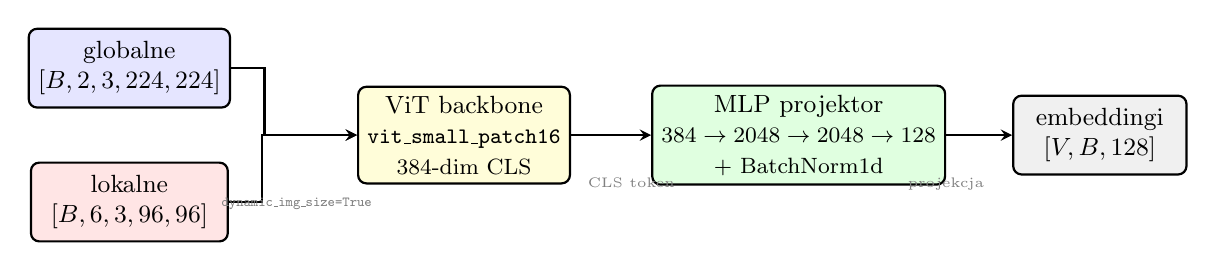
\begin{tikzpicture}[>=stealth, scale=0.85,
  box/.style={draw, thick, rounded corners=3pt, minimum height=1cm,
              align=center, font=\small}]

  % Widoki wejściowe
  \node[box, fill=blue!10, minimum width=2.5cm] (gin) at (0, 1.5)
    {globalne\\$[B, 2, 3, 224, 224]$};
  \node[box, fill=red!10, minimum width=2.5cm] (lin) at (0, -0.5)
    {lokalne\\$[B, 6, 3, 96, 96]$};

  % ViT backbone
  \node[box, fill=yellow!15, minimum width=2.2cm] (vit) at (5, 0.5)
    {ViT backbone\\{\footnotesize\texttt{vit\_small\_patch16}}\\{\footnotesize $384$-dim CLS}};

  % Projektor MLP
  \node[box, fill=green!12, minimum width=2.5cm] (proj) at (10, 0.5)
    {MLP projektor\\{\footnotesize $384 \to 2048 \to 2048 \to 128$}\\{\footnotesize + BatchNorm1d}};

  % Wyjście
  \node[box, fill=gray!12, minimum width=2.2cm] (out) at (14.5, 0.5)
    {embeddingi\\$[V, B, 128]$};

  % Strzałki
  \draw[->, thick] (gin.east) -- ++(0.5,0) |- (vit.west);
  \draw[->, thick] (lin.east) -- ++(0.5,0) |- (vit.west);
  \draw[->, thick] (vit) -- (proj);
  \draw[->, thick] (proj) -- (out);

  % Opis pod strzałkami
  \node[below, font=\tiny, gray] at (2.5, -0.3)
    {\texttt{dynamic\_img\_size=True}};
  \node[below, font=\tiny, gray] at (7.5, -0.0)
    {CLS token};
  \node[below, font=\tiny, gray] at (12.2, -0.0)
    {projekcja};
\end{tikzpicture}
\end{center}

\textbf{Kluczowe detale:}

\begin{itemize}[leftmargin=2em]
  \item \textbf{Różne rozdzielczości} ---
    widoki globalne ($224^2$) i~lokalne ($96^2$) mają
    \textbf{różną liczbę patchy}:
    $(224/16)^2 = 196$ vs $(96/16)^2 = 36$.
    ViT obsługuje to dzięki \texttt{dynamic\_img\_size=True}
    w~bibliotece \texttt{timm} --- pozycyjne embeddingi
    są interpolowane do aktualnej rozdzielczości.

  \item \textbf{Wspólne wagi} --- ten sam ViT i~ten sam projektor
    przetwarzają \textit{wszystkie} widoki.
    Nie ma osobnych sieci dla globalnych i~lokalnych.

  \item \textbf{Kształt wyjściowy} ---
    $[V, B, d] = [8, B, 128]$, gdzie $V = V_g + V_l = 2 + 6 = 8$.
    Pierwszy wymiar indeksuje widoki, drugi --- obrazy w~batchu,
    trzeci --- $128$-wymiarową przestrzeń embeddingów.

  \item \textbf{Projektor MLP} --- trójwarstwowy:
    $384 \xrightarrow{\text{Linear}} 2048
     \xrightarrow{\text{BN+ReLU}} 2048
     \xrightarrow{\text{BN+ReLU}} 128$.
    BatchNorm1d po każdej warstwie ukrytej
    stabilizuje trening.
    SIGReg i~loss predykcyjny operują
    na $128$-wymiarowych projekcjach, nie na surowych cechach $384$-dim.
\end{itemize}

%% --- 6. Podsumowanie ---
\subsubsection{Podsumowanie: widoki globalne vs lokalne}

\begin{center}
\renewcommand{\arraystretch}{1.4}
\begin{tabular}{l c c}
\toprule
& \textbf{Widoki globalne} & \textbf{Widoki lokalne} \\
\midrule
\textbf{Liczba}             & $V_g = 2$ & $V_l = 6$ \\
\textbf{Rozdzielczość}      & $224 \times 224$ & $96 \times 96$ \\
\textbf{Skala kadrowania}   & $[0{.}3,\; 1{.}0]$ & $[0{.}05,\; 0{.}3]$ \\
\textbf{Patche ViT}         & $14 \times 14 = 196$ & $6 \times 6 = 36$ \\
\textbf{Źródło (obrazy)}    & ta sama klatka & ta sama klatka \\
\textbf{Źródło (wideo)}     & klatka anchor $t$ & sąsiedzi $t \pm 15$ \\
\textbf{Rola w~lossie}      & centroid $\boldsymbol{\mu}_n$
                             & zbliżają się do $\boldsymbol{\mu}_n$ \\
\textbf{Intuicja}           & ``co to jest?'' (kontekst)
                             & ``jak wygląda z~bliska?'' (detale) \\
\bottomrule
\end{tabular}
\end{center}

\begin{keyinsight}[Wielowidokowość = inwariantność + hierarchia]
Widoki globalne dają \textbf{stabilny punkt odniesienia}
(centroid), a~widoki lokalne \textbf{wymuszają},
by sieć rozumiała detale w~kontekście całości.
Razem tworzą sygnał uczący, który produkuje embeddingi
\textbf{inwariantne} wobec skali, perspektywy i~(w~wideo) czasu
--- bez heurystyk typu momentum encoder czy stop-gradient.
\end{keyinsight}

\subsection{Czytanie wzoru (\ref{eq:lejepa}) od lewej do prawej}

Teraz czytamy wzór po polsku, symbol po symbolu:

\begin{tcolorbox}[colback=blue!4, colframe=blue!60!black, breakable,
  title={\textbf{Wzór (\ref{eq:lejepa}) --- jak go przeczytać}}]

\[
\mathcal{L}_{\text{LeJEPA}} =
\underbrace{\frac{\lambda}{V} \sum_{v=1}^{V} \mathrm{SIGReg}\!\left(\{\mathbf{z}_{n,v}\}_{n=1}^B\right)}_{\text{część A}}
+
\underbrace{\frac{1-\lambda}{B} \sum_{n=1}^{B} \mathcal{L}_{\text{pred}}^{(V_g)}\!\left(\{\mathbf{z}_{n,v}\}_{v=1}^V\right)}_{\text{część B}}
\]

\textbf{Część A --- regularyzacja SIGReg:}

\medskip
Czytamy: \textit{``Weź wagę $\lambda$, podziel przez liczbę widoków $V$,
i~dla każdego widoku $v$ od 1 do $V$ policz SIGReg
na zbiorze embeddingów wszystkich $B$ obrazów w~tym widoku.''}

\begin{enumerate}[leftmargin=2em]
  \item Fiksujemy widok $v$ (np.\ ``widok globalny nr~1'').
  \item Zbieramy embeddingi \textbf{tego widoku} ze~wszystkich obrazów w~batchu:
        $\{\mathbf{z}_{1,v},\; \mathbf{z}_{2,v},\; \ldots,\; \mathbf{z}_{B,v}\}$
        --- to $B$ wektorów w~$\mathbb{R}^d$.
  \item Sprawdzamy SIGRegiem: czy te $B$ wektorów tworzą
        rozkład $\mathcal{N}(\mathbf{0}, \mathbf{I})$?
  \item Powtarzamy dla każdego widoku $v = 1, \ldots, V$ i~uśredniamy ($\div V$).
  \item Mnożymy przez wagę $\lambda$ (typowo $0{.}05$).
\end{enumerate}

\textbf{Intuicja}: regularyzacja sprawdza \textit{kolumnami} ---
``czy chmura embeddingów z~każdego widoku wygląda jak izotropowy Gauss?''

\bigskip
\textbf{Część B --- predykcja:}

\medskip
Czytamy: \textit{``Weź wagę $(1-\lambda)$, podziel przez liczbę obrazów $B$,
i~dla każdego obrazu $n$ policz loss predykcyjny na wszystkich jego widokach.''}

\begin{enumerate}[leftmargin=2em]
  \item Fiksujemy obraz $n$ (np.\ ``zdjęcie kota nr~17'').
  \item Zbieramy embeddingi \textbf{tego obrazu} ze~wszystkich widoków:
        $\{\mathbf{z}_{n,1},\; \mathbf{z}_{n,2},\; \ldots,\; \mathbf{z}_{n,V}\}$.
  \item Liczymy centroid z~widoków globalnych:
        $\boldsymbol{\mu}_n = \frac{1}{V_g}(\mathbf{z}_{n,1} + \mathbf{z}_{n,2})$.
  \item Mierzymy, jak daleko każdy widok jest od centroidu:
        $\|\boldsymbol{\mu}_n - \mathbf{z}_{n,v'}\|_2^2$.
  \item Uśredniamy po widokach ($\div V$) i~po obrazach ($\div B$).
  \item Mnożymy przez wagę $(1 - \lambda)$ (typowo $0{.}95$).
\end{enumerate}

\textbf{Intuicja}: predykcja sprawdza \textit{wierszami} ---
``czy różne widoki tego samego obrazu dają podobne embeddingi?''
\end{tcolorbox}

\subsubsection*{Skąd biorą się widoki? Obrazy vs wideo}

Pojęcie ``widoku'' (view) oznacza coś innego w~zależności od danych:

\begin{tcolorbox}[colback=orange!5, colframe=orange!70!black, breakable,
  title={\textbf{Widoki --- obrazy (np.\ ImageNet)}}]
Mamy jeden obraz, np.\ zdjęcie kota.
\textbf{Wszystkie} widoki powstają z~\textbf{tego samego} zdjęcia
przez \textbf{augmentacje} --- losowe kadrowania, obroty, zmiany kolorów:

\begin{center}
\begin{tikzpicture}[>=stealth, scale=0.85]
  % Oryginalny obraz
  \draw[thick] (0,0) rectangle (3,3);
  \node at (1.5,1.5) {\large obraz $\mathbf{x}_n$};
  \node[below] at (1.5,-0.2) {\small (np.\ zdjęcie kota)};

  % Strzałki
  \draw[->, thick] (3.3, 2.5) -- (5.0, 3.2);
  \draw[->, thick] (3.3, 2.0) -- (5.0, 2.0);
  \draw[->, thick] (3.3, 1.5) -- (5.0, 1.0);
  \draw[->, thick] (3.3, 0.8) -- (5.0, -0.2);

  % Widoki globalne
  \draw[blue!70!black, thick] (5.0, 2.7) rectangle (7.5, 3.7);
  \node[blue!70!black] at (6.25, 3.2) {\small glob.\ $224^2$};

  \draw[blue!70!black, thick] (5.0, 1.5) rectangle (7.5, 2.5);
  \node[blue!70!black] at (6.25, 2.0) {\small glob.\ $224^2$};

  % Widoki lokalne
  \draw[red!70!black, thick] (5.0, 0.5) rectangle (6.8, 1.3);
  \node[red!70!black] at (5.9, 0.9) {\small lok.\ $96^2$};

  \draw[red!70!black, thick] (5.0, -0.7) rectangle (6.8, 0.1);
  \node[red!70!black] at (5.9, -0.3) {\small lok.\ $96^2$};

  \node at (7.5, 0.2) {\small $\ldots$};

  % Etykiety
  \node[blue!70!black, anchor=west] at (7.7, 3.2) {\small $V_g = 2$};
  \node[red!70!black, anchor=west] at (7.1, -0.3) {\small $V_l = 6$};

  % Opis
  \node[anchor=west, align=left] at (8.2, 1.5) {\small Ten sam kot,\\
    \small różne wycinki\\
    \small \textbf{tej samej} klatki};
\end{tikzpicture}
\end{center}

Widoki globalne i~lokalne to \textbf{różne wycinki tej samej fotografii}.
Sieć uczy się: ``duży wycinek kota i~mały wycinek ucha
$\Rightarrow$ to~ten sam kot $\Rightarrow$ bliskie embeddingi.''
\end{tcolorbox}

\begin{tcolorbox}[colback=violet!5, colframe=violet!70!black, breakable,
  title={\textbf{Widoki --- wideo (np.\ chirurgia katarakty)}}]
Mamy \textbf{film}, nie pojedyncze zdjęcie.
Widoki pochodzą z~\textbf{różnych klatek}:

\begin{center}
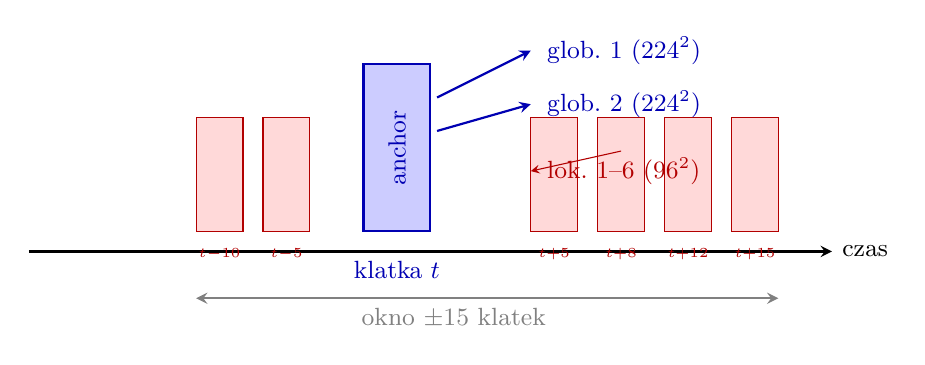
\begin{tikzpicture}[>=stealth, scale=0.85]
  % Oś czasu
  \draw[->, thick] (0,0) -- (12,0) node[right] {\small czas};

  % Klatka anchor
  \fill[blue!20] (5.0, 0.3) rectangle (6.0, 2.8);
  \draw[blue!70!black, thick] (5.0, 0.3) rectangle (6.0, 2.8);
  \node[blue!70!black, rotate=90] at (5.5, 1.55) {\small anchor};
  \node[below, blue!70!black] at (5.5, 0.0) {\small klatka $t$};

  % Widoki globalne z anchora
  \draw[->, blue!70!black, thick] (6.1, 2.3) -- (7.5, 3.0);
  \draw[->, blue!70!black, thick] (6.1, 1.8) -- (7.5, 2.2);
  \node[blue!70!black, anchor=west] at (7.6, 3.0) {\small glob.\ 1 ($224^2$)};
  \node[blue!70!black, anchor=west] at (7.6, 2.2) {\small glob.\ 2 ($224^2$)};

  % Klatki sąsiednie
  \foreach \x/\lab in {2.5/$t{-}10$, 3.5/$t{-}5$, 7.5/$t{+}5$, 8.5/$t{+}8$, 9.5/$t{+}12$, 10.5/$t{+}15$} {
    \fill[red!15] (\x, 0.3) rectangle ({\x+0.7}, 2.0);
    \draw[red!70!black] (\x, 0.3) rectangle ({\x+0.7}, 2.0);
    \node[below, red!70!black, font=\tiny] at ({\x+0.35}, 0.2) {\lab};
  }

  % Strzałki od sąsiadów do lokalnych widoków
  \node[red!70!black, anchor=west] at (7.6, 1.2) {\small lok.\ 1--6 ($96^2$)};
  \draw[->, red!70!black] (8.85, 1.5) -- (7.5, 1.2);

  % Okno ±15
  \draw[<->, gray, thick] (2.5, -0.7) -- (10.5+0.7, -0.7);
  \node[gray, below] at (6.35, -0.7) {\small okno $\pm 15$ klatek};
\end{tikzpicture}
\end{center}

\begin{itemize}[leftmargin=2em]
  \item \textbf{Widoki globalne} ($V_g = 2$): duże kadrowania z~\textbf{klatki anchor}
        (jeden konkretny moment $t$) --- te same piksele, różne wycinki.
  \item \textbf{Widoki lokalne} ($V_l = 6$): małe kadrowania z~\textbf{sąsiednich klatek}
        w~oknie $\pm 15$ klatek wokół anchora
        (np.\ klatka z~$t - 5$, $t + 8$, $t + 12$, \ldots).
\end{itemize}

\textbf{Dlaczego to działa?}
W~filmie chirurgicznym klatki oddalone o~kilka--kilkanaście klatek
pokazują \textbf{tę samą scenę}: to samo narzędzie, ta sama tkanka,
lekko zmieniony kąt.
Sieć uczy się: ``klatka z~sekundy 5.0 i~klatka z~sekundy 5.3
przedstawiają ten sam etap operacji $\Rightarrow$ bliskie embeddingi.''

\medskip
\textbf{Przewaga nad obrazami}: w~wideo nie potrzebujemy sztucznych augmentacji
(obroty, zmiana kolorów), bo \textbf{sam upływ czasu} naturalnie generuje
różne widoki tej samej sceny --- zmienia się oświetlenie,
kąt mikroskopu, pozycja narzędzia.
To są \textbf{prawdziwe} transformacje, nie syntetyczne.
\end{tcolorbox}

\subsection{Czytanie wzoru (\ref{eq:pred_loss}) --- loss predykcyjny}

\begin{tcolorbox}[colback=orange!5, colframe=orange!70!black, breakable,
  title={\textbf{Wzór (\ref{eq:pred_loss}) --- co dokładnie liczy $\mathcal{L}_{\text{pred}}$}}]

\[
\mathcal{L}_{\text{pred}} = \frac{1}{V}\sum_{v'=1}^{V}
\left\|\boldsymbol{\mu}_n - \mathbf{z}_{n,v'}\right\|_2^2,
\qquad
\boldsymbol{\mu}_n \triangleq \frac{1}{V_g}\sum_{v=1}^{V_g} \mathbf{z}_{n,v}
\]

\textbf{Krok 1 --- oblicz centroid $\boldsymbol{\mu}_n$:}

Bierzemy tylko widoki \textbf{globalne} (duże kadrowania) i~liczymy ich średnią:
\[
\boldsymbol{\mu}_n = \frac{\mathbf{z}_{n,1} + \mathbf{z}_{n,2}}{2}
\quad\text{(bo $V_g = 2$)}
\]

Centroid to ``punkt środkowy'' --- najlepsza reprezentacja tego, co sieć ``myśli''
o~obrazie $n$ na podstawie globalnych widoków.

\textbf{Dlaczego tylko globalne?}
Globalne widoki widzą duży fragment obrazu $\Rightarrow$ mają najwięcej informacji
$\Rightarrow$ są najbardziej wiarygodnym punktem odniesienia.

\bigskip
\textbf{Krok 2 --- zmierz odległość każdego widoku od centroidu:}

Dla \textit{każdego} widoku $v'$ (globalnego i~lokalnego) liczymy:
\[
\left\|\boldsymbol{\mu}_n - \mathbf{z}_{n,v'}\right\|_2^2
= \sum_{i=1}^{d} \left(\mu_{n,i} - z_{n,v',i}\right)^2
\]

To jest zwykły \textbf{kwadrat odległości euklidesowej} w~$\mathbb{R}^d$
--- suma kwadratów różnic po każdej współrzędnej.

\bigskip
\textbf{Krok 3 --- uśrednij:}

$\frac{1}{V}\sum_{v'=1}^{V}$ --- średnia z~$V$ odległości.

\medskip
\textbf{Co to wymusza?}
Jeśli ten sam kot sfotografowany z~bliska i~z~daleka daje
\textit{bliskie} embeddingi (mała odległość od centroidu),
to sieć nauczyła się rozpoznawać ``kotowość'' niezależnie od kadrowania.
\end{tcolorbox}

\subsection{Konkretny przykład liczbowy}

Weźmy $B = 2$ obrazy, $V_g = 2$ widoki globalne, $V_l = 1$ widok lokalny
($V = 3$), $d = 2$ wymiary (zamiast 128, dla prostoty), $\lambda = 0.05$.

\medskip
\textbf{Embeddingi} (sieć wypluwa):
\[
\begin{array}{c|ccc}
 & v=1 \text{ (glob.)} & v=2 \text{ (glob.)} & v=3 \text{ (lok.)} \\
\hline
\text{obraz } n=1 & \mathbf{z}_{1,1} = (1.0,\; 0.5) & \mathbf{z}_{1,2} = (0.8,\; 0.7)
  & \mathbf{z}_{1,3} = (1.3,\; 0.3) \\
\text{obraz } n=2 & \mathbf{z}_{2,1} = (-0.6,\; 1.2) & \mathbf{z}_{2,2} = (-0.4,\; 0.8)
  & \mathbf{z}_{2,3} = (-0.8,\; 1.0)
\end{array}
\]

\textbf{Część B --- predykcja (czytamy wierszami):}

Centroidy z~widoków globalnych:
\begin{align*}
\boldsymbol{\mu}_1 &= \tfrac{1}{2}\bigl((1.0, 0.5) + (0.8, 0.7)\bigr) = (0.9,\; 0.6) \\
\boldsymbol{\mu}_2 &= \tfrac{1}{2}\bigl((-0.6, 1.2) + (-0.4, 0.8)\bigr) = (-0.5,\; 1.0)
\end{align*}

Odległości od centroidu (obraz 1):
\begin{align*}
\|\boldsymbol{\mu}_1 - \mathbf{z}_{1,1}\|^2 &= (0.9-1.0)^2 + (0.6-0.5)^2 = 0.01 + 0.01 = 0.02 \\
\|\boldsymbol{\mu}_1 - \mathbf{z}_{1,2}\|^2 &= (0.9-0.8)^2 + (0.6-0.7)^2 = 0.01 + 0.01 = 0.02 \\
\|\boldsymbol{\mu}_1 - \mathbf{z}_{1,3}\|^2 &= (0.9-1.3)^2 + (0.6-0.3)^2 = 0.16 + 0.09 = 0.25
\end{align*}
\[
\mathcal{L}_{\text{pred}}^{(1)} = \frac{0.02 + 0.02 + 0.25}{3} = 0.097
\]

Analogicznie dla obrazu 2: powiedzmy $\mathcal{L}_{\text{pred}}^{(2)} = 0.063$.

\[
\text{Część B} = \frac{1 - 0.05}{2}(0.097 + 0.063) = \frac{0.95}{2} \cdot 0.16 = 0.076
\]

\textbf{Część A --- regularyzacja (czytamy kolumnami):}

Dla widoku $v = 1$: zbieramy $\{\mathbf{z}_{1,1}, \mathbf{z}_{2,1}\} = \{(1.0, 0.5),\; (-0.6, 1.2)\}$
i~sprawdzamy SIGRegiem, czy to $\mathcal{N}(\mathbf{0}, \mathbf{I})$.
Powiedzmy $\mathrm{SIGReg}_1 = 0.31$.
Analogicznie dla $v = 2, 3$.

\[
\text{Część A} = \frac{0.05}{3}(0.31 + 0.28 + 0.45) = \frac{0.05}{3} \cdot 1.04 = 0.017
\]

\textbf{Pełny loss:}
\[
\mathcal{L}_{\text{LeJEPA}} = \underbrace{0.017}_{\text{SIGReg}} + \underbrace{0.076}_{\text{predykcja}} = 0.093
\]

\begin{keyinsight}[Dwa cele, jedna liczba]
Widzimy, że predykcja dominuje ($0.076$ vs $0.017$) --- tak ma być przy $\lambda = 0.05$.
Sieć skupia się na \textbf{semantycznej spójności} widoków (``ten sam kot $\Rightarrow$ bliskie wektory''),
a~SIGReg działa w~tle jako \textbf{strażnik} (``ale nie kolapsuj do jednego punktu --- rozpychaj się gaussowsko!'').
\end{keyinsight}

\subsection{Podsumowanie: regularyzacja vs predykcja}

\begin{center}
\renewcommand{\arraystretch}{1.3}
\begin{tabular}{lcc}
\toprule
& \textbf{Regularyzacja (SIGReg)} & \textbf{Predykcja} \\
\midrule
\textbf{Iteruje po} & widokach ($v$) & obrazach ($n$) \\
\textbf{Zbiera} & embeddingi jednego widoku z~$B$ obrazów & embeddingi jednego obrazu z~$V$ widoków \\
\textbf{Sprawdza} & ``czy rozkład $\approx \mathcal{N}(\mathbf{0}, \mathbf{I})$?'' & ``czy widoki się zgadzają?'' \\
\textbf{Chroni przed} & kolapsem (wszystko $\to$ jeden punkt) & chaosem (losowe embeddingi) \\
\textbf{Waga} & $\lambda = 0.05$ (5\%) & $1 - \lambda = 0.95$ (95\%) \\
\bottomrule
\end{tabular}
\end{center}

%% ============================================================
\subsection{Od filmu do klasyfikacji --- cały pipeline end-to-end}
\label{sec:end_to_end}
%% ============================================================

Mamy teraz wszystkie elementy.
Zobaczmy, jak \textbf{cały system} działa od surowego wideo
chirurgii katarakty do konkretnego zastosowania klinicznego
--- rozpoznawania narzędzi chirurgicznych na klatce.

Pipeline składa się z~dwóch niezależnych faz:
\textbf{pretraining} (samouczenie bez etykiet)
i~\textbf{downstream} (wykorzystanie wyuczonych reprezentacji).

%% --- Faza 1: Pretraining ---
\subsubsection{Faza 1: Pretraining LeJEPA (samouczenie)}
\label{sec:e2e_pretraining}

\begin{center}
\begin{tikzpicture}[>=stealth, scale=0.82,
  box/.style={draw, thick, rounded corners=3pt, minimum height=1.0cm,
              align=center, font=\small},
  bigbox/.style={draw, thick, rounded corners=5pt, minimum height=1.2cm,
              align=center, font=\small}]

  %% --- Etap 1: Dane ---
  \node[bigbox, fill=gray!12, minimum width=2.5cm] (data) at (0, 0)
    {\textbf{Wideo}\\{\footnotesize zbiór filmów operacji}\\
     {\footnotesize \textit{bez etykiet}}};

  %% --- Etap 2: Sampling ---
  \node[box, fill=yellow!12, minimum width=2.5cm] (sample) at (4.5, 0)
    {\textbf{Sampling}\\{\footnotesize anchor $t$}\\
     {\footnotesize $\pm 15$ klatek}};

  %% --- Etap 3: Widoki ---
  \node[box, fill=blue!10, minimum width=1.5cm] (gv) at (8.5, 0.9)
    {glob.\ $\times 2$\\{\footnotesize $224^2$}};
  \node[box, fill=red!10, minimum width=1.5cm] (lv) at (8.5, -0.9)
    {lok.\ $\times 6$\\{\footnotesize $96^2$}};

  %% --- Etap 4: Enkoder ---
  \node[box, fill=orange!12, minimum width=2.0cm] (enc) at (12, 0)
    {\textbf{ViT}\\{\footnotesize 384-dim}\\{\footnotesize + MLP $\to$ 128}};

  %% --- Etap 5: Loss ---
  \node[bigbox, fill=lejepaBlue!12, minimum width=2.5cm] (loss) at (16, 0)
    {\textbf{Loss LeJEPA}\\{\footnotesize $\lambda \cdot \text{SIGReg}$}\\
     {\footnotesize $+ (1{-}\lambda) \cdot \text{pred}$}};

  %% Strzałki
  \draw[->, thick] (data) -- (sample);
  \draw[->, thick, blue!70!black] (sample) -- ++(1.5, 0) |- (gv);
  \draw[->, thick, red!70!black] (sample) -- ++(1.5, 0) |- (lv);
  \draw[->, thick] (gv) -- ++(1.2, 0) |- (enc);
  \draw[->, thick] (lv) -- ++(1.2, 0) |- (enc);
  \draw[->, thick] (enc) -- (loss);

  %% Strzałka powrotna (gradient)
  \draw[->, thick, dashed, lejepaRed]
    (loss.south) -- ++(0, -1.2) -| (enc.south)
    node[pos=0.25, below, font=\footnotesize, lejepaRed] {$\nabla_\theta \mathcal{L}$ (backprop)};

\end{tikzpicture}
\end{center}

\textbf{Krok po kroku --- jedna iteracja treningu:}

\begin{enumerate}[leftmargin=2em]
  \item \textbf{Załaduj batch filmów.}
    Z~kolekcji nagrań operacji katarakty wybieramy $B$ filmów
    (np.\ $B = 64$). Filmy nie mają \textit{żadnych} etykiet
    --- nie wiemy, co jest na której klatce.

  \item \textbf{Wylosuj klatki anchor.}
    Z~każdego filmu losujemy jedną klatkę $t$
    (z~marginesem $\pm 15$ od brzegów).

  \item \textbf{Wygeneruj widoki.}
    \begin{itemize}[leftmargin=1.5em]
      \item Z~klatki $t$: \textbf{2 widoki globalne}
            ($224 \times 224$, skala $0{.}3$--$1{.}0$).
      \item Z~6 losowych sąsiadów $t \pm 15$: \textbf{6 widoków lokalnych}
            ($96 \times 96$, skala $0{.}05$--$0{.}3$).
    \end{itemize}
    Każdy widok przechodzi augmentacje chirurgiczne
    (zredukowany jitter, rotacja $\pm 15^{\circ}$, bez solaryzacji).

  \item \textbf{Forward pass.}
    Wszystkie $8$ widoków przechodzą przez \textbf{ten sam} ViT
    ($\to$ CLS token $384$-dim) i~\textbf{ten sam} MLP projektor
    ($\to$ embedding $128$-dim).
    Wynik: tensor $[8, B, 128]$.

  \item \textbf{Oblicz loss.}
    \begin{itemize}[leftmargin=1.5em]
      \item \textbf{SIGReg} (5\%): dla każdego z~8 widoków zbierz
            $B$ embeddingów i~sprawdź, czy tworzą
            $\mathcal{N}(\mathbf{0}, \mathbf{I})$.
      \item \textbf{Predykcja} (95\%): dla każdego z~$B$ filmów policz
            centroid z~widoków globalnych i~zmierz odległość
            wszystkich 8 widoków od centroidu.
    \end{itemize}
    Suma ważona daje skalar $\mathcal{L}_{\text{LeJEPA}}$.

  \item \textbf{Backpropagation.}
    Gradient $\nabla_\theta \mathcal{L}$ przepływa wstecz
    przez projektor i~ViT.
    Optymalizator (AdamW, lr $= 3 \times 10^{-4}$, weight decay $= 0{.}05$)
    aktualizuje wagi $\theta$.
    \textbf{Nie ma} momentum encodera, stop-gradientu, ani EMA
    --- gradient przepływa bezpośrednio przez całą sieć.

  \item \textbf{Powtórz} przez $N$ epok (np.\ 100--300).
\end{enumerate}

\begin{keyinsight}[Co się dzieje w~trakcie treningu?]
Na początku ViT produkuje \textbf{losowe} embeddingi
--- widoki tego samego fragmentu operacji mają odległe wektory,
a~SIGReg jest daleki od $\mathcal{N}(\mathbf{0}, \mathbf{I})$.

Z~każdą epoką:
\begin{itemize}[leftmargin=1.5em]
  \item loss predykcyjny \textbf{ściąga} embeddingi widoków tego samego filmu
        do wspólnego centroidu --- sieć uczy się, że klatka $t$ i~klatka $t+5$
        to ta sama scena,
  \item SIGReg \textbf{rozpycha} embeddingi różnych filmów
        --- sieć uczy się, że ``fazoemulsyfikacja'' $\neq$ ``hydrodyssekcja''.
\end{itemize}

Po treningu ViT backbone produkuje \textbf{semantycznie bogate}
$384$-wymiarowe reprezentacje, w~których bliskość
wektorów odpowiada bliskości semantycznej scen chirurgicznych.
\end{keyinsight}

\textbf{Co otrzymujemy na końcu pretreningu?}

Wytrenowany model ViT --- plik \texttt{checkpoint.pt}
zawierający wagi backbone'u.
Projektor MLP \textbf{odrzucamy} --- służył tylko do treningu
(projekcja $384 \to 128$ była potrzebna dla SIGReg,
ale $384$-wymiarowe cechy z~backbone'u
są bogatsze i~lepsze do zadań downstream).

%% --- Faza 2: Downstream ---
\subsubsection{Faza 2: Wykorzystanie wyuczonej wiedzy (downstream)}
\label{sec:e2e_downstream}

Wytrenowany backbone to \textbf{uniwersalny ekstraktor cech}
--- ``rozumie'' chirurgię, ale nie wie jeszcze,
jakie konkretne pytanie mu zadajemy.
Aby go wykorzystać, dokładamy niewielką głowicę (head)
i~trenujemy ją na \textit{etykietowanych} danych.

\medskip
Pokażemy to na przykładzie \textbf{rozpoznawania narzędzi chirurgicznych}
na klatkach wideo:

\begin{center}
\begin{tikzpicture}[>=stealth, scale=0.82,
  box/.style={draw, thick, rounded corners=3pt, minimum height=1.0cm,
              align=center, font=\small}]

  %% Wejście
  \node[box, fill=gray!12, minimum width=2.5cm] (img) at (0, 0)
    {\textbf{Klatka wideo}\\{\footnotesize nowa, nigdy nie widziana}};

  %% Zamrożony ViT
  \node[box, fill=orange!12, minimum width=2.5cm] (vit) at (5.5, 0)
    {\textbf{ViT backbone}\\{\footnotesize (zamrożony)}\\
     {\footnotesize $\to$ cechy $384$-dim}};

  %% Głowica
  \node[box, fill=lejepaGreen!15, minimum width=2.5cm] (head) at (11, 0)
    {\textbf{Głowica}\\{\footnotesize Linear $384 \to K$}\\
     {\footnotesize (trenowana)}};

  %% Wyjście
  \node[box, fill=lejepaBlue!12, minimum width=2.5cm] (out) at (16, 0)
    {\textbf{Predykcja}\\{\footnotesize ``phaco handpiece''}\\
     {\footnotesize $p = 0{.}94$}};

  %% Strzałki
  \draw[->, thick] (img) -- (vit);
  \draw[->, thick] (vit) -- (head)
    node[midway, above, font=\footnotesize] {$\mathbf{h} \in \mathbb{R}^{384}$};
  \draw[->, thick] (head) -- (out)
    node[midway, above, font=\footnotesize] {softmax};

  %% Zamek (zamrożone wagi)
  \node[font=\large] at (5.5, -1.2) {\footnotesize zamrożone wagi z~pretreningu};

  %% Strzałka gradientu (tylko do głowicy)
  \draw[->, thick, dashed, lejepaGreen!70!black]
    (out.south) -- ++(0, -0.8) -| (head.south)
    node[pos=0.25, below, font=\footnotesize, lejepaGreen!70!black]
    {gradient (tylko głowica)};
\end{tikzpicture}
\end{center}

Istnieją trzy główne sposoby wykorzystania pretrenowanego backbone'u:

\bigskip
\textbf{(A) Linear probing --- liniowa głowica na zamrożonym backbone'u}

To najprostszy i~najbardziej \textit{diagnostyczny} sposób ewaluacji:

\begin{enumerate}[leftmargin=2em]
  \item \textbf{Zamroź} wagi ViT (żaden gradient nie przepływa do backbone'u).
  \item Dodaj jedną warstwę \texttt{Linear(384, $K$)}, gdzie $K$ = liczba klas
        narzędzi (np.\ $K = 21$ w~zbiorze CaDIS:
        \textit{phaco handpiece, capsulorhexis cystotome, lens injector, \ldots}).
  \item Trenuj \textbf{tylko} tę warstwę na etykietowanych klatkach
        (np.\ 5000 klatek z~ręcznymi adnotacjami).
  \item Ewaluacja: softmax daje rozkład prawdopodobieństwa
        po $K$ klasach narzędzi.
\end{enumerate}

\textbf{Dlaczego to jest dobry test?}
Jeśli \textit{jedna} warstwa liniowa potrafi na podstawie
$384$-wymiarowych cech poprawnie rozpoznawać narzędzia,
to znaczy, że backbone \textbf{już wie}, czym różni się
phaco handpiece od irygacji --- musi to tylko ``powiedzieć''.
Cechy są \textbf{liniowo separowalne}.

\bigskip
\textbf{(B) $k$-NN --- klasyfikacja bez żadnego trenowania}

Jeszcze prostszy test, który nie wymaga \textit{żadnego} dodatkowego trenowania:

\begin{enumerate}[leftmargin=2em]
  \item Przepuść wszystkie etykietowane klatki przez zamrożony ViT
        $\to$ baza wektorów $\{(\mathbf{h}_i, y_i)\}$
        (cecha $384$-dim + etykieta).
  \item Dla nowej, niewidzianej klatki oblicz cechę $\mathbf{h}_{\text{query}}$.
  \item Znajdź $k$ najbliższych sąsiadów (np.\ $k = 20$)
        w~bazie wg odległości euklidesowej lub kosinusowej.
  \item Predykcja = klasa najczęstsza wśród $k$ sąsiadów
        (głosowanie większościowe).
\end{enumerate}

\textbf{Intuicja}: jeśli cechy LeJEPA są dobre,
to klatka z~phaco handpiece będzie blisko \textit{innych} klatek
z~phaco handpiece w~$384$-wymiarowej przestrzeni.
$k$-NN bezpośrednio testuje jakość \textbf{geometrii} tej przestrzeni.

\bigskip
\textbf{(C) Fine-tuning --- pełna adaptacja}

Gdy zależy nam na maksymalnej dokładności, nie tylko na~diagnozie jakości cech:

\begin{enumerate}[leftmargin=2em]
  \item Inicjalizuj ViT wagami z~pretreningu.
  \item Dodaj głowicę klasyfikacyjną (jak w~linear probing).
  \item Trenuj \textbf{całą sieć} end-to-end, ale z~niskim learning rate
        dla backbone'u (np.\ $10\times$ mniejszy niż dla głowicy),
        aby nie zniszczyć wyuczonych reprezentacji.
\end{enumerate}

\textbf{Przewaga nad treningiem od zera}: backbone \textit{startuje}
z~sensownymi cechami chirurgicznymi, więc potrzebuje
\textbf{znacznie mniej} etykietowanych danych i~epok,
aby osiągnąć dobrą dokładność.
Typowo: trening od zera wymaga ${\sim}50\text{k}$ etykietowanych klatek;
po pretreningu LeJEPA wystarczy ${\sim}5\text{k}$.

\begin{tcolorbox}[colback=violet!5, colframe=violet!70!black, breakable,
  title={\textbf{Podsumowanie: dwie fazy, dwa cele}}]

\begin{center}
\renewcommand{\arraystretch}{1.4}
\begin{tabular}{l c c}
\toprule
& \textbf{Faza 1: Pretraining} & \textbf{Faza 2: Downstream} \\
\midrule
\textbf{Dane}           & filmy \textit{bez etykiet}
                         & klatki \textit{z~etykietami} \\
\textbf{Ilość danych}   & dużo (setki godzin)
                         & mało (tysiące klatek) \\
\textbf{Co się trenuje} & cały ViT + projektor
                         & głowica (lub cały ViT z~niskim lr) \\
\textbf{Loss}           & $\lambda \cdot \text{SIGReg} + (1{-}\lambda) \cdot \text{pred}$
                         & cross-entropy \\
\textbf{Cel}            & ``zrozum chirurgię''
                         & ``odpowiedz na konkretne pytanie'' \\
\textbf{Wynik}          & uniwersalny ekstraktor cech
                         & klasyfikator / detektor / segmentor \\
\bottomrule
\end{tabular}
\end{center}

\medskip
\textbf{Kluczowa idea}: ogromną większość wiedzy sieć zdobywa
w~fazie~1, oglądając setki godzin operacji \textit{bez nadzoru}.
Faza~2 tylko \textbf{kanalizuje} tę wiedzę w~stronę konkretnego zadania
--- i~dlatego wystarcza jej niewielka ilość etykietowanych danych.

To jest istota \textbf{self-supervised learning}:
zamień tanie, nieetykietowane dane na drogą, semantyczną reprezentację
--- a~potem wykorzystaj ją tanio.
\end{tcolorbox}

